\documentclass[11pt,xcolor={svgnames},aspectratio=169,usepdftitle=false,notheorems]{beamer}

%===========================================================
% DOCUMENT
%===========================================================
\usepackage{rafa_style_beamer}
\addbibresource{../matlab_intro.bib}
\title{Introduction to Matlab}
\subtitle{Lesson 03 --- Basics of Root Finding, Numerical Differentiation, and Integration}

\author{Rafael Serrano-Quintero}

\institute{Department of Economics \\ University of Barcelona}
\date{}

\begin{document}

\VerbatimFootnotes

\maketitle

\section{Basics of Root Finding}

\begin{frame}
  \frametitle{Root Finding --- The Problem}
Say we want to find all $x$ such that $f(x) = 0$. If:
\begin{itemize}
  \item $f(x) = ax^2 + bx + c \Rightarrow x = \frac{-b \pm \sqrt{b^2 - 4ac}}{2a}$ solves the problem for any $\{a,b,c\}\in\mathbb{R}$ {\tiny (and $a\neq 0$)}.
  \item Sometimes, we cannot solve explicitly for $x$ even in the realm of polynomials!
  \item If $f(x) = ax^5 + bx^4 + cx^3 + dx^2 + ex + f$ where $\{a,b,c,d,e,f\}\in\mathbb{R}$ we do not have an explicit formula to solve for $f(x) = 0$. Neither for polynomials of order $\geq 5$. But we know \alert{\textbf{such roots do exist!}} {\tiny see \href{https://en.wikipedia.org/wiki/Fundamental_theorem_of_algebra}{Fundamental Theorem of Algebra}}
  \item Then... what should we do?
\end{itemize}
\end{frame}

\begin{frame}
  \frametitle{Root Finding --- Intuition}
Say we have a nonlinear $f(x)$ for which we know at least one root exists.
\begin{itemize}
  \item Suppose we know the root is \textit{somewhere around} $x_0$.
  \item Starting from $x_0$ construct a sequence of $\{x_k\}$ hoping it converges to a root $x^*$ such that $f(x^*) = 0$.
\end{itemize}
This highlights two important features of root finding \textit{algorithms}:
\begin{itemize}
  \item \alert{\textbf{Convergence:}} is the sequence $\{f(x_k)\}$ getting \textit{closer} to $f(x^*) = 0$?
  \item \alert{\textbf{Stopping criteria:}} how do we know we are \textit{close enough}?
\end{itemize}
We can discuss convergence and stopping criteria in each method studied.
\end{frame}

\subsection{Bisection Method}

\begin{frame}[c]
  \frametitle{Bisection Method --- Intuition}
 \begin{itemize}
  \item Say you have a phone book (old school, I know). You need to find Garc\'ia in there.
  \item What method do you use?
  \pause
  \begin{enumerate}
    \item Turn page by page until you find it.
    \pause
    \item Turn every two pages. 
    \pause
    \item Open by the middle, check if G is left or right. Discard one half. Repeat until you find it.
  \end{enumerate}
 \end{itemize} 
\end{frame}

\begin{frame}
  \frametitle{Bisection Method --- Intuition}
Consider $f : \mathbb{R} \mapsto \mathbb{R}$ where the problem is $f(x^*) = 0$. Suppose $f(x)$ is continuous in $[a,b]$ and we know $\exists x^*\in[a,b]$ {\tiny (The ideas presented generalize to $n$ dimensions)}

\begin{itemize}
  \item \alert{\textbf{Bisect}} the interval $[a,b]$ and take the middle point $c = \frac{a + b}{2}$. If $f(c) = 0$ we are done. Otherwise, $x^*$ must be in either $[a,c]$ or $[c,b]$.
  \item Find the one that contains $x^*$ and bisect again. \alert{\textbf{How?!?}}
  \item Continue until the interval is as small as the accuracy desired.
\end{itemize}
\end{frame}

\begin{frame}
  \frametitle{Bisection Method --- Intuition}
\begin{theorem}[\href{https://en.wikipedia.org/wiki/Intermediate_value_theorem}{The Intermediate Value Theorem (IVT)}]
Suppose $f(x)$ is continuous on $[a,b]\subseteq\mathbb{R}$ and $M$ in between $f(a)$ and $f(b)$. Then, there is at least one $c\in(a,b)$ such that $f(c) = M$. If $f(a) < 0 < f(b)$ then, there is a root $x = c$ such that $f(c) = 0$.
\end{theorem}

\begin{itemize}
  \item If $f(c) < 0$, by the IVT, the root of $f(x)$ must be in $[c,b]$
  \item Otherwise, if $f(c) > 0$, by the IVT, the root must be in $[a,c]$
  \item Note that this algorithm finds \alert{\textbf{a zero, not all zeros}} of $f(x)$
\end{itemize}
\end{frame}

\begin{frame}
  \frametitle{Bisection Method --- the Algorithm}
  \begin{enumerate}
    \item Initialize and bracket a zero. {\tiny \alert{\textbf{(Initial guess)}}}
    \begin{itemize}
      \item Find $x^L < x^R$ such that $f(x^L)f(x^R) < 0$
      \item Choose stopping rule parameters
    \end{itemize}
    \item Compute $x^M = \frac{x^L + x^R}{2}$
    \item Test if $x^M$ is a root. If so, stop. {\tiny \alert{\textbf{(Test if it is an acceptable solution)}}}
    \item If $x^M$ is not a root, refine interval. {\tiny \alert{\textbf{(Iterate)}}}
    \begin{itemize}
      \item If $f(x^M)f(x^L) < 0$ let $x^R = x^M$ and leave $x^L$ unchanged.
      \item Else, $x^L = x^M$ and leave $x^R$ unchanged.
    \end{itemize}
    \item Repeat until the stopping rule tells us to stop.
  \end{enumerate}
\end{frame}

\begin{frame}
  \frametitle{Bisection Method --- Remarks}
\begin{itemize}
  \item The algorithm \alert{\textbf{always converges}} (we always find a solution).
  \item Convergence can be very slow but it is a very \alert{\textbf{reliable}} method.
  \item We have not yet defined proper stopping criteria.
\end{itemize}
\alert{\textbf{Stopping Criteria:}}
\begin{enumerate}
  \item The value of the function is lower than or equal to the tolerance $\lvert f(x^M) \rvert \leq \delta$.
  \item The length of the interval is very small. $(x^R - x^L) / (1 + \lvert x^L \rvert + \lvert x^R \rvert) \leq \varepsilon$.
  \item The number of iterations is larger than a predetermined number $N$.
\end{enumerate}
\end{frame}


\subsection{Newton-Raphson Method}

\begin{frame}
  \frametitle{Newton-Raphson Method --- Intuition}
\begin{itemize}
  \item When using bisection, we have only assumed continuity of $f(x)$
  \item However, bisection can be slow. Newton-Raphson's method uses properties of \alert{\textbf{smooth}} functions.
  \item This method is faster but may not always converge.
  \item \alert{\textbf{Key idea:}} approximate $f(x)$ by a succession of linear functions. Approximate zeros with the zeros of the linear approximations.
\end{itemize}
\end{frame}

\begin{frame}
  \frametitle{Newton-Raphson --- Preliminaries}
\begin{definition}
A number $c$ is a \alert{\textbf{fixed point}} of $g(x)$ if $g(c) = c$.
\end{definition}
\begin{itemize}
  \item Note then that $f(x) = 0 \Rightarrow f(x) = x - g(x) = 0$ and any fixed point $c$ of $g(x)$ is a root of $f(x)$ because
  \[
  f(c) = c - g(c) = c - c = 0
  \]
  \item Finding a root of $f(x) \equiv$ find a fixed point of  $x = g(x)$ such that $f(x) = 0$
  \item \alert{\textbf{Problem:}} How to rewrite $f(x) = 0$ as $x = g(x)$?
\end{itemize}
\end{frame}

\begin{frame}
  \frametitle{Newton-Raphson --- Preliminaries}
\begin{itemize}
  \item We can know existence, uniqueness, and convergence (see Theorem \ref{thm:fixed_point}). However, verifying Assumption 1 is not easy.
  \item This method chooses $g(x)$ as $g(x) = x - \frac{f(x)}{f'(x)}$ and the iteration scheme is:
  \begin{equation}
  x_{k+1} = x_k - \frac{f(x_k)}{f'(x_k)} \label{eqn:newton_iteration}
  \end{equation}
  \item For this choice, we can state sufficient conditions for convergence.
\end{itemize}

\begin{theorem}
Suppose $f(x)$ is $\mathcal{C}^2$ and that $f(x^*) = 0$. If $x_0$ is sufficiently close to $x^*$, $f'(x)\neq 0$, and $\lvert f''(x) / f'(x)\rvert < \infty$, the iteration scheme defined by \eqref{eqn:newton_iteration} converges to $x^*$.
\end{theorem}
\end{frame}

\begin{frame}
  \frametitle{Newton-Raphson --- Preliminaries}
Where does the choice for $g(x)$ come from? Recall \href{https://en.wikipedia.org/wiki/Taylor's_theorem}{Taylor's Theorem} and linearly approximate $f(x)$ around $x_k$:
\[
p(x) = f(x_k) + (x - x_k)f'(x_k)
\]
\begin{itemize}
  \item $p(x)$ and $f(x)$ are tangent at $x_k$ and close in the neighborhood of $x_k$
  \item Solving for a zero of $p(x) \Rightarrow x = x_k - \frac{f(x_k)}{f'(x_k)}$ which is the iteration scheme \eqref{eqn:newton_iteration}
  \item Which yields our new guess for $x_{k+1}$
\end{itemize}
\end{frame}

\begin{frame}
  \frametitle{Newton-Raphson --- The Algorithm}
\begin{enumerate}
  \item Choose stopping criterion parameters $\{\varepsilon, \delta, N\}$, and a starting point $x_0$. Set the iteration counter $k = 0$.
  \item Compute next iteration using \eqref{eqn:newton_iteration}
  \item Test for convergence. If either one of the following:
  \begin{itemize}
    \item $\lvert x_k - x_{k+1} \rvert \leq \varepsilon (1 + \lvert x_{k+1}\rvert)$
    \item $\lvert f(x_{k+1}) \rvert \leq \delta$
    \item $k > N$
  \end{itemize}
  \textbf{Stop}
  \item Repeat until one of the convergence criteria is satisfied.
\end{enumerate}
\end{frame}

\begin{frame}
  \frametitle{Newton-Raphson --- Remarks}
\begin{itemize}
  \item The method is not guaranteed to converge. If after $N$ iterations we have not found a root, the method failed.
  \item Note that we rely on our initial guess being \alert{\textbf{close}} to the root. If we are far, we may very well fail.
  \item For some functions and starting points, we may enter an infinite loop. The sequence of iterations will oscillate without converging to any value.
  \item Even when passing both $\varepsilon$ and $\delta$ tests, we may not have found a zero.
\end{itemize}
\end{frame}

\begin{frame}[fragile]
  \frametitle{Newton-Raphson --- Some Issues} 
  \begin{columns}
  \begin{column}{0.39\textwidth}
  \begin{itemize}
    \item Consider $f(x) = x^6$
    \item $x_{k+1} = (5/6)x_k$
    \item Still far after $100$ iterations!
  \end{itemize}
  \end{column}
  \begin{column}{0.6\textwidth}
    \begin{figure}
      \centering
      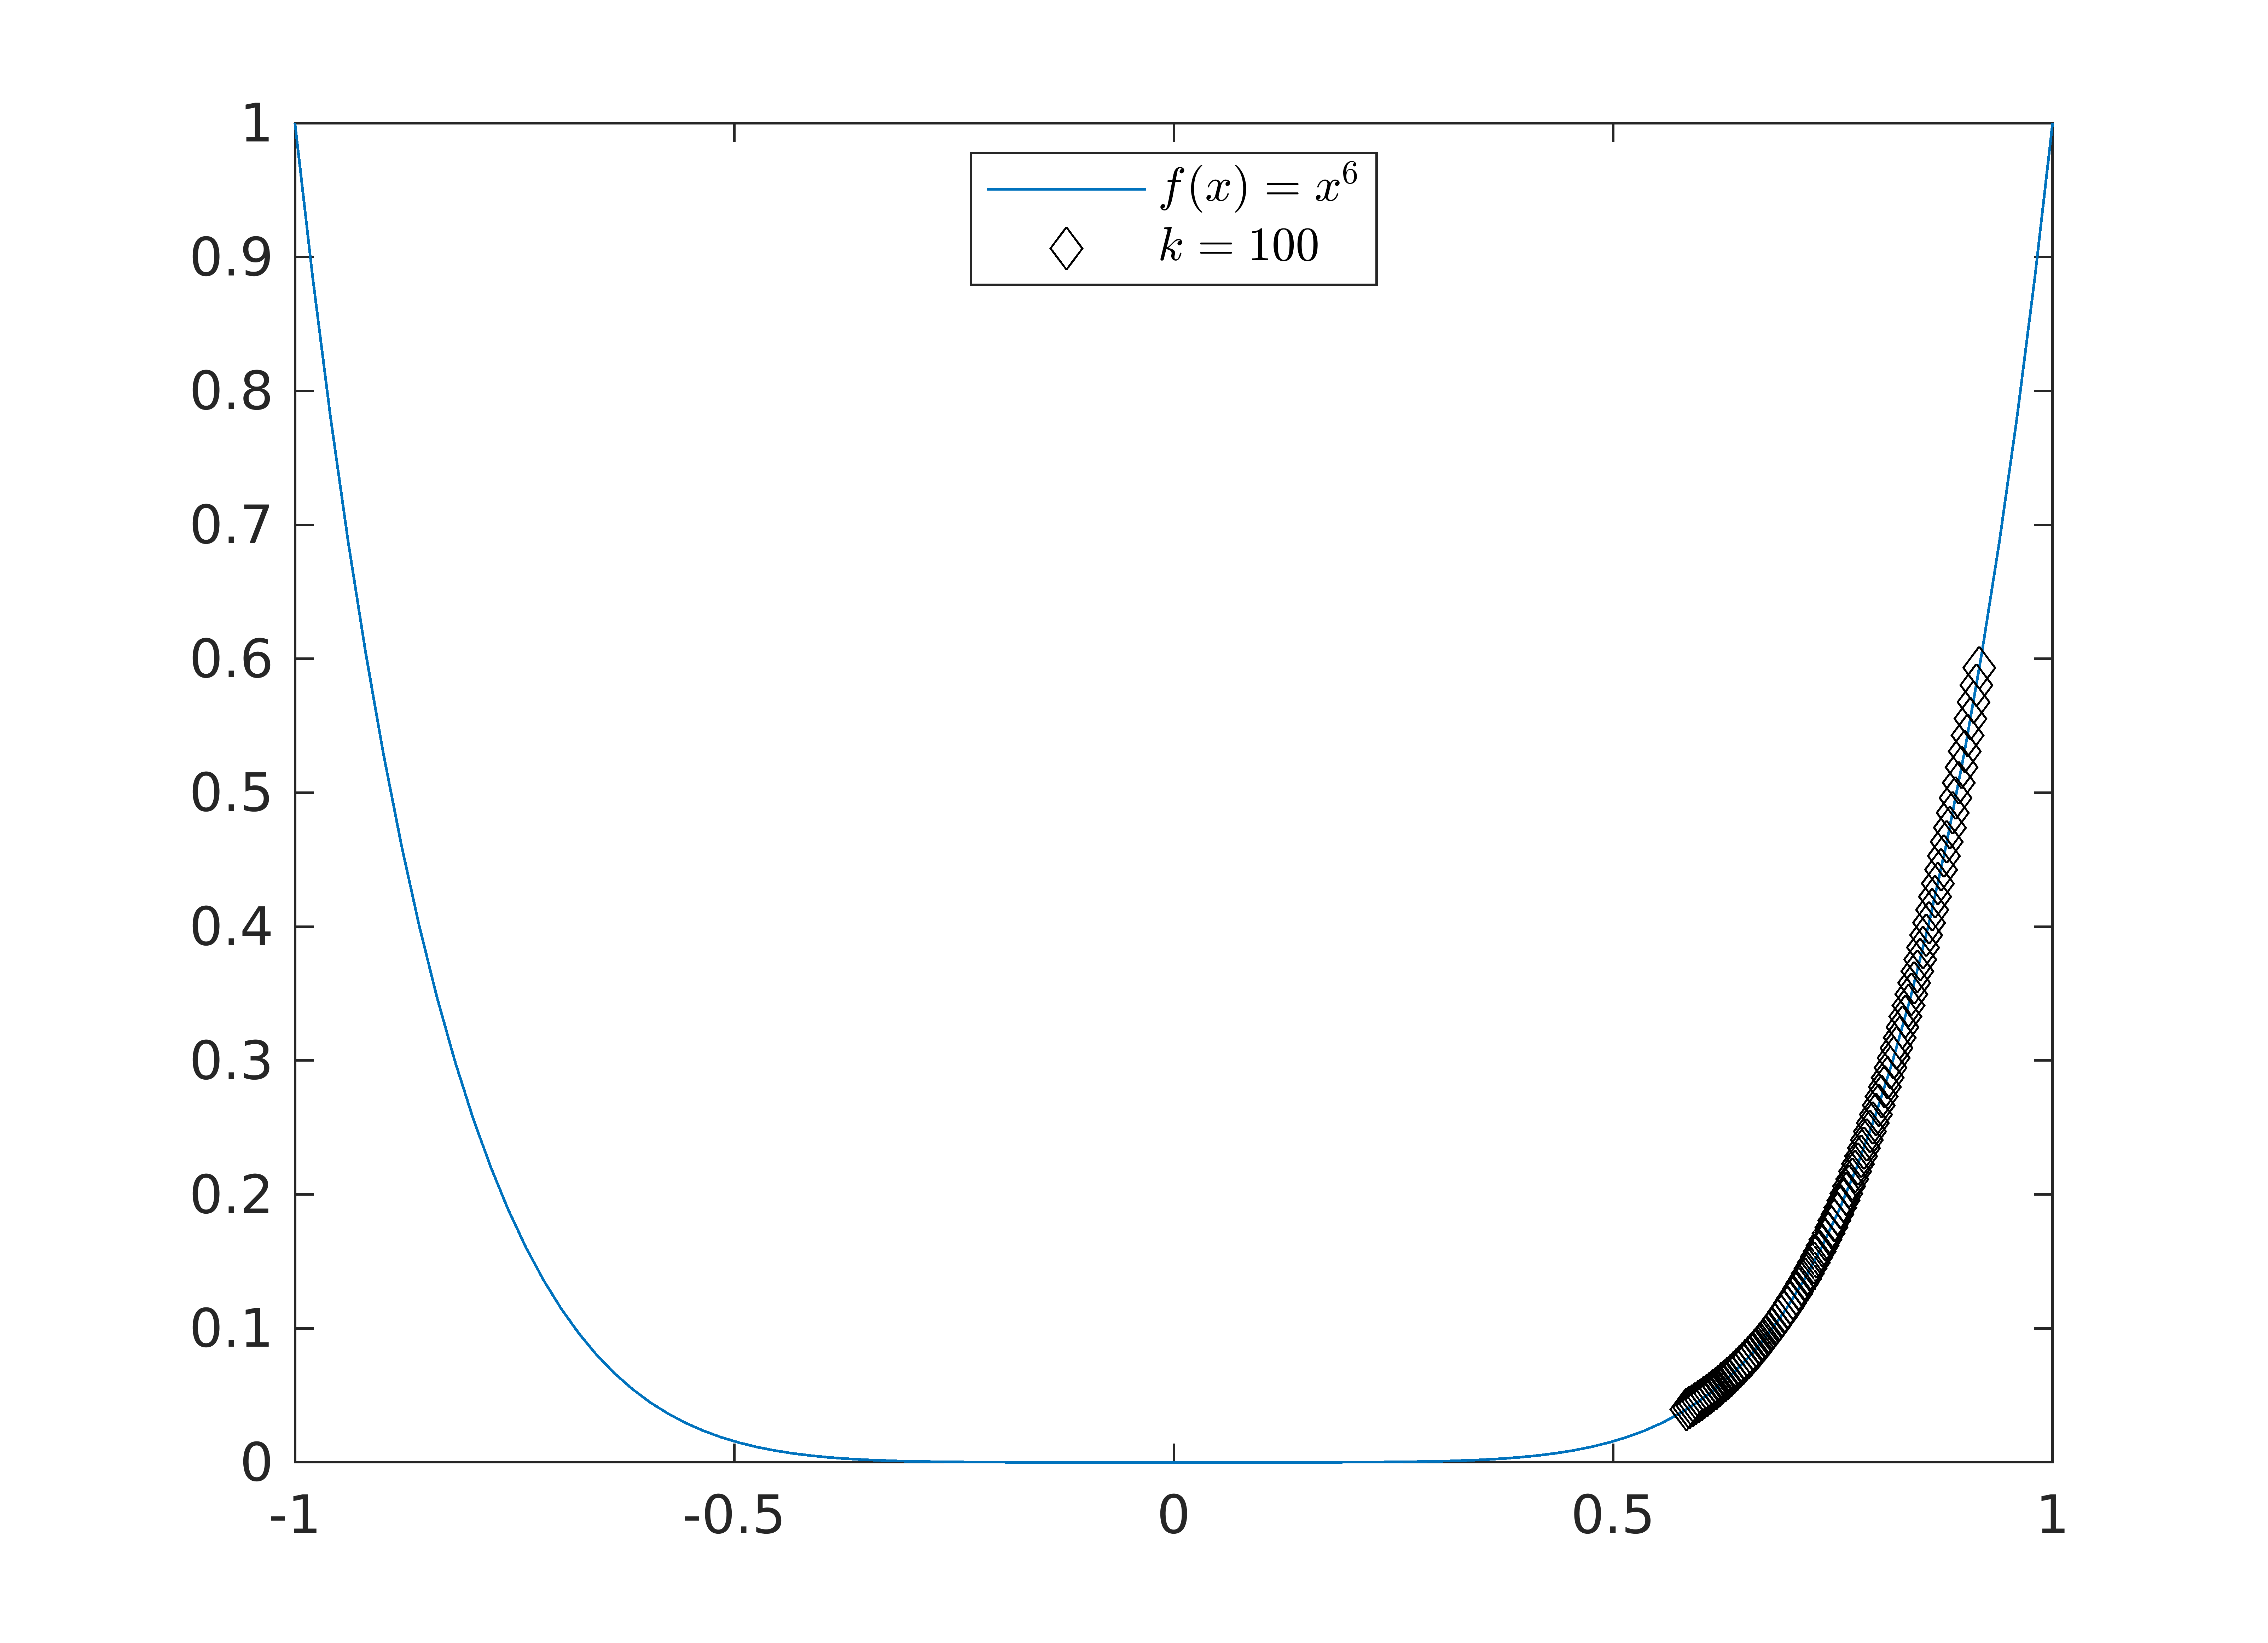
\includegraphics[width = \textwidth]{../figures/newton_convergence_issues.png}
      \caption{Convergence Issues with Newton-Raphson}
      \label{fig:newton_convergence}
    \end{figure}
\end{column}
\end{columns}
\end{frame}

\begin{frame}
  \frametitle{Root Finding in Matlab}
\begin{itemize}
  \item We have learned two very powerful methods to find roots
  \item Matlab has implemented \href{https://www.mathworks.com/help/matlab/ref/fzero.html}{\texttt{fzero}} for such problems.
  \item This function combines bisection with secant and inverse quadratic interpolation (we have not seen this but many ideas apply).
  \item Another function is \href{https://www.mathworks.com/help/matlab/ref/roots.html}{\texttt{roots}} which finds the roots of polynomials.
  \item Familiarize yourselves with these functions and compare them with the methods we have implemented.
\end{itemize}
\end{frame}

\subsection{Solving Equations in Practice}

\begin{frame}[c]
  \frametitle{Example --- Arrow-Debreu Equilibrium}
  \begin{itemize}
    \item Say we have two agents $A$ and $B$, and two goods $1$ and $2$. The preferences of the agents are
      \[
        u_A(x_{1,A}, x_{2,A}) = \left( x_{1,A} \right)^{\alpha} \left( x_{2,A} \right)^{1 - \alpha} \qquad u_B(x_{1,B}, x_{2,B}) = \left( x_{1,B} \right)^{\beta} \left( x_{2,B} \right)^{1 - \beta}
      \]
    \item Their initial endowments are $\{\omega_{1,i}, \omega_{2,i}\}$
    \item In equilibrium, it must be that $m_i = p_1 \omega_{1,i} + p_2\omega_{2,i}$.
  \end{itemize}
\end{frame}

\begin{frame}[c]
  \frametitle{Example --- Arrow-Debreu Equilibrium}
 \begin{itemize}
  \item The demand functions are given by:
  \begin{align}
    x_{1,A}\left( p_1, p_2, m_A \right) & = \alpha\frac{m_A}{p_1} \label{eq:demand_1A} \\
    x_{2,A}\left( p_1, p_2, m_A \right) & = \left( 1 - \alpha \right)\frac{m_A}{p_2} \label{eq:demand_2A} \\ 
    x_{1,B}\left( p_1, p_2, m_B \right) & = \beta\frac{m_B}{p_1} \label{eq:demand_1B} \\
    x_{2,B}\left( p_1, p_2, m_B \right) & = \left( 1 - \beta \right)\frac{m_B}{p_2}  \label{eq:demand_2B}
  \end{align}
  \item Define the excess demand for goods $1$ and $2$ as 
    \begin{align}
      z_1(p_1, p_2) & = x_{1,A}\left( p_1, p_2, m_A \right) + x_{1,B}\left( p_1, p_2, m_B \right) - \omega_{1,A} - \omega_{1,B} \\
      z_2(p_2, p_2) & = x_{2,A}\left( p_2, p_2, m_A \right) + x_{2,B}\left( p_2, p_2, m_B \right) - \omega_{2,A} - \omega_{2,B}
    \end{align}
 \end{itemize} 
\end{frame}

\begin{frame}[c]
  \frametitle{Example --- Arrow-Debreu Equilibrium}
    \begin{align*}
      z_1(p_1, p_2) & = x_{1,A}\left( p_1, p_2, m_A \right) + x_{1,B}\left( p_1, p_2, m_B \right) - \omega_{1,A} - \omega_{1,B} \\
      z_2(p_2, p_2) & = x_{2,A}\left( p_2, p_2, m_A \right) + x_{2,B}\left( p_2, p_2, m_B \right) - \omega_{2,A} - \omega_{2,B}
    \end{align*}
\begin{itemize}
  \item Substituting the demand functions \eqref{eq:demand_1A}-\eqref{eq:demand_2B} and dividing by $p_2$ (we only care about relative prices, check Walras' Law if you don't see this).
\end{itemize}
\begin{gather*}
  z_1(p_1, 1) = \alpha \frac{p_1\omega_{1,A} + \omega_{2,A}}{p_1} + \beta \frac{p_1\omega_{1,B} + \omega_{2,B}}{p_1} - \omega_{1,A} - \omega_{1,B} \\
  z_2(p_1, 1) = (1 - \alpha) \left(p_1\omega_{1,A} + \omega_{2,A}\right) + (1 - \beta) \left(p_1\omega_{1,B} + \omega_{2,B}\right) - \omega_{2,A} - \omega_{2,B}
\end{gather*}
\end{frame}

\begin{frame}[c]
  \frametitle{Example --- Arrow-Debreu Equilibrium}
\begin{gather}
  z_1(p_1, 1) = \alpha \frac{p_1\omega_{1,A} + \omega_{2,A}}{p_1} + \beta \frac{p_1\omega_{1,B} + \omega_{2,B}}{p_1} - \omega_{1,A} - \omega_{1,B} \\
  z_2(p_1, 1) = (1 - \alpha) \left(p_1\omega_{1,A} + \omega_{2,A}\right) + (1 - \beta) \left(p_1\omega_{1,B} + \omega_{2,B}\right) - \omega_{2,A} - \omega_{2,B}
\end{gather}
\begin{itemize}
  \item An equilibrium is then a price $p_1$ such that $z_1(p_1,1) = z_2(p_2,1) = 0$. 
  \item We can use any of the two to get the solution for $p_1$. 
  \item The analytical solution is 
\end{itemize}
\[
  p_1^* = \frac{\alpha\omega_{2,A} + \beta\omega_{2,B}}{(1 - \alpha)\omega_{1,A} + (1 - \beta)\omega_{1,B}} 
\]
\end{frame}

\section{Basics of Numerical Differentiation}

\begin{frame}
  \frametitle{Numerical Differentiation --- Why?}
\begin{itemize}
  \item Numerical evaluation of the derivatives in economics is \alert{\textbf{crucial!}}
  \begin{itemize}
    \item Newton-Raphson, optimization, ODEs \ldots
  \end{itemize}
  \item Sometimes, it is difficult or cumbersome to compute derivatives analytically. In those cases, we turn to \textit{numerical} evaluation of derivatives.
  \item Recall the definition of the derivative of a function
  \[
  f'(x) = \lim_{h\rightarrow 0} \frac{f(x+h) - f(x)}{h} \text{ \tiny (can recall why?) }
  \]
  we can approximate $f'(x)$ by choosing a \textit{step size} $h$.
  \item That is called, \textit{finite differences}.
\end{itemize}
\end{frame}

\begin{frame}
  \frametitle{Numerical Differentiation --- An Example}
Take the function 
\[
f(x) = x^3 - 6x^2 + 11x - 6
\]
\begin{itemize}
  \item The analytical derivative is 
  \[
  f'(x) = 3x^2 - 12x + 11
  \]
  \item Let's approximate the derivative by using finite differences in Matlab with on $x\in [-5,5]$
  \item Compute $dy$ as $f(x+h) - f(x)$ for a fixed $h$ and $dx = h$.
  \item The numerical derivative is given by $f'(x) = \frac{dy}{dx}$.
\end{itemize}
\end{frame}

\begin{frame}[fragile]
  \frametitle{Numerical Differentiation --- An Example}
\begin{columns}
\begin{column}{0.38\textwidth}
{\footnotesize As $h\rightarrow 0$, the derivative converges.}
\begin{lstlisting}
N = 10;
x = linspace(-5,5,N);
h = 1;
% Numerical derivative
dy = myf(x+h) - myf(x);
dx = h.*ones(size(dy));
fp_num = dy./dx;
\end{lstlisting}
\end{column}
\begin{column}{0.61\textwidth}
  \begin{figure}
    \centering
    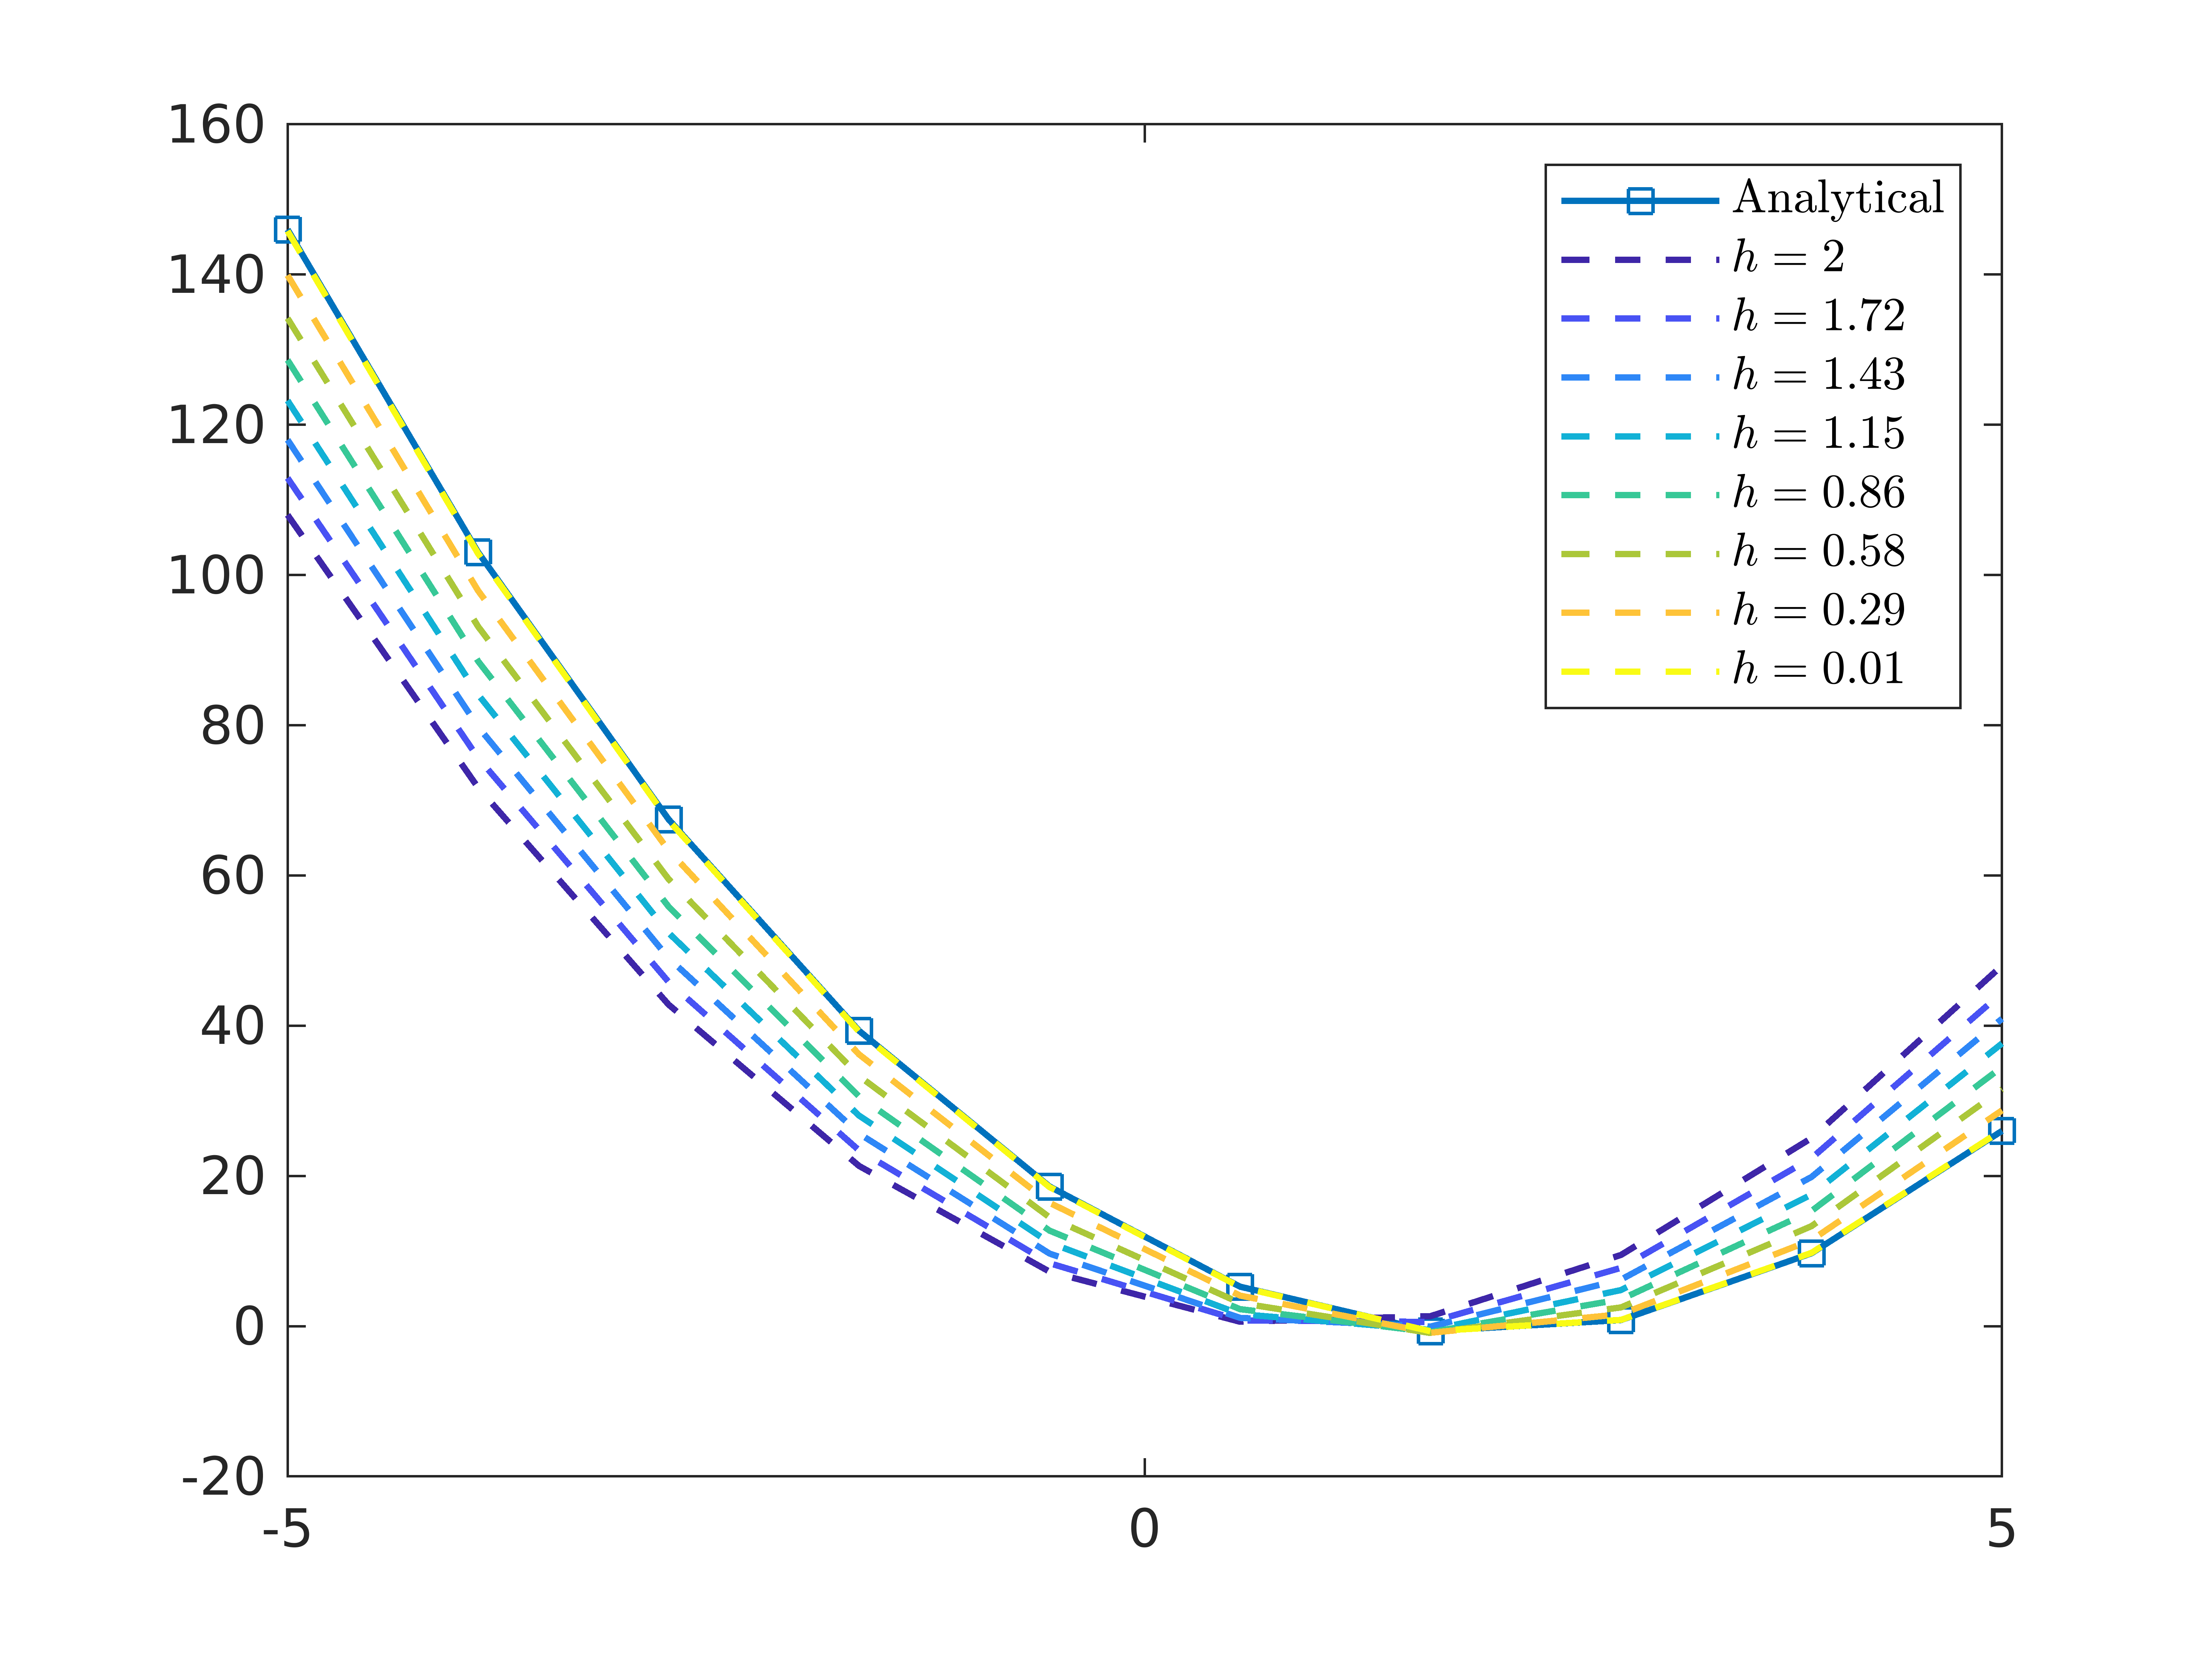
\includegraphics[width = \textwidth]{../figures/finite_differences.png}
    \caption{Accuracy of Finite Difference}
    \label{fig:finite_differences}
  \end{figure}
\end{column}
\end{columns}
\end{frame}

\begin{frame}
  \frametitle{Numerical Differentiation --- An Application to ODEs}
\begin{itemize}
  \item The \href{https://en.wikipedia.org/wiki/Solow–Swan_model}{Solow-Swan growth model} finds an equilibrium solution by solving the ODE
  \begin{equation}
    \dot{k} = \frac{dk}{dt} = s f(k) - \delta k
    \label{eqn:solow_capital}
  \end{equation}
  where $k$ is physical capital, $f(k)$ is the production function, $s$ is an exogenous savings rate, and $\delta$ is the depreciation rate of capital.
  \item Approximate $k(t)$ at $N$ discrete points in the time dimension $t^n, n = 1,\ldots, N$ and denote the distance between the points by $h$.
  \item Approximate $\dot{k}$ using finite differences $\dot{k}(t^n) \approx \frac{k^{n+1} - k^n}{h}$
  \item We can compute $k(t^{n+1})$ recursively given $h$ and $k(0) = k_0$ 
  \[
  k(t^{n+1}) = k(t^{n}) + h \left(s f(k^n) - \delta k^n\right)
  \]
\end{itemize}
\end{frame}

\begin{frame}
  \frametitle{Numerical Differentiation --- An Application to ODEs}
  \begin{minipage}{0.3\textwidth}
  \begin{itemize}
    \item Horizon $T = 70$
    \item $N = 10$ points.
    \item Compare with \href{https://www.mathworks.com/help/matlab/ref/ode45.html}{\texttt{ode45}} and analytical solution.
  \end{itemize}
  \end{minipage}
\begin{minipage}{0.65\textwidth}
  \begin{figure}
    \centering
    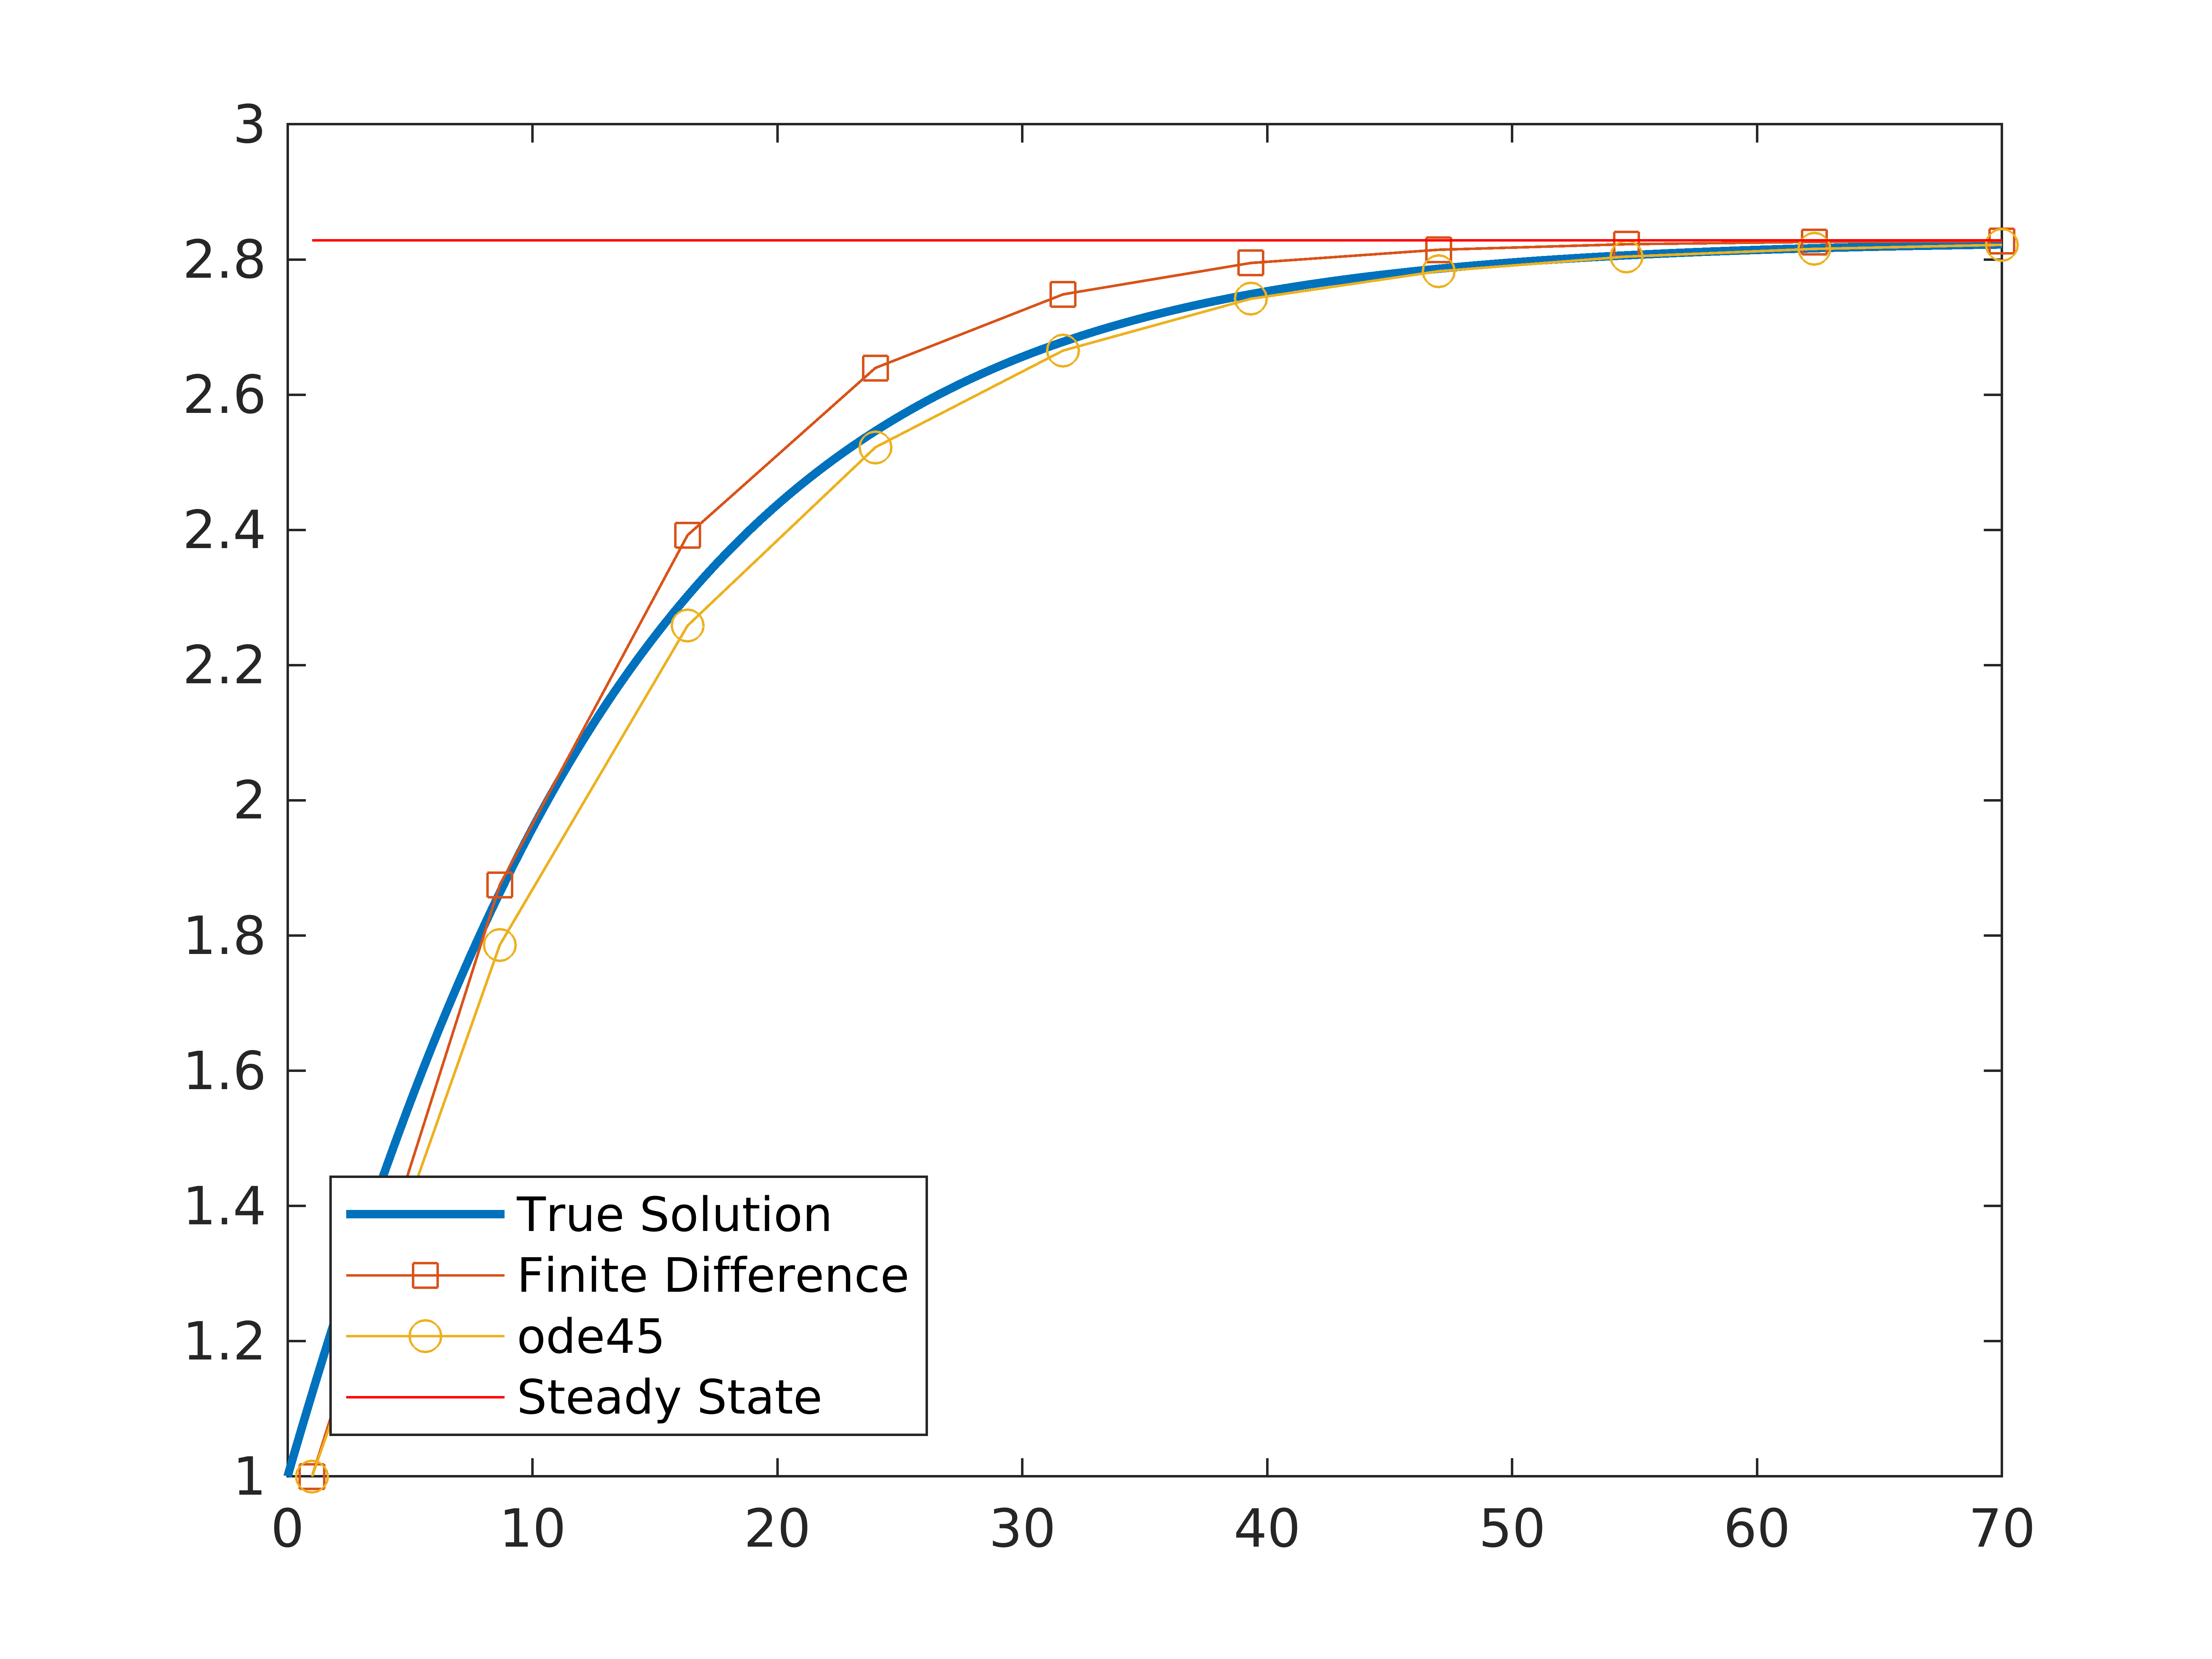
\includegraphics[width = \textwidth]{../figures/solow_solution.png}
    \caption{Trajectory for $k(t)$}
    \label{fig:solow_finitedifferences}
  \end{figure}
\end{minipage}
\end{frame}

\begin{frame}
  \frametitle{Symbolic and Automatic Differentiation}
\begin{itemize}
  \item \href{https://www.mathworks.com/help/symbolic/diff.html\#btwol6i-2}{Symbolic differentiation} applies the rules of derivatives to symbolic expressions. What we humans do.
  \item \href{https://en.wikipedia.org/wiki/Automatic_differentiation}{Automatic differentiation} breaks codes into smaller sections and applies the chain rule \parencite[See Chapter~4]{kwon2019julia}.
  \item The advantage of automatic differentiation is that computes \alert{\textbf{analytical}} derivatives at the same cost. No error!
  \item Automatic differentiation evaluates expressions numerically early, symbolic differentiation at the end.
  \item Thus, symbolic is more costly. Check \href{https://www.mathworks.com/help/deeplearning/ug/deep-learning-with-automatic-differentiation-in-matlab.html}{Matlab's documentation}
\end{itemize}
\end{frame}

\section{Basics of Numerical Integration}

\begin{frame}
  \frametitle{Numerical Integration --- Why?}
\begin{itemize}
  \item Numerical evaluation of integrals in economics is ubiquitous.
  \begin{itemize}
    \item Expectations, posteriors in Bayesian statistics, ODEs (again\ldots)
  \end{itemize}
  \item Again, sometimes it is computationally expensive to compute integrals.
  \item The definite integral of $f(x)$ is the area under its graph.
  \item Furthermore, the definition of the definite integral involves an infinte sum (\href{https://en.wikipedia.org/wiki/Riemann_sum}{Riemann Sum}).
  \item We will approximate integrals by computing sums in particular ways.
\end{itemize}
\end{frame}

\begin{frame}
  \frametitle{Numerical Integration --- Preliminaries}
\begin{definition}
  Let $f : [a,b]\mapsto\mathbb{R}$. Let $\mathcal{P}$ and $\mathcal{T}$ be a \alert{\textbf{partition pair}} such that $\mathcal{P},\mathcal{T}\subset [a,b]$ where $\mathcal{P} = \{x_0,\ldots,x_n\}$, $\mathcal{T} = \{t_1,\ldots,t_n\}$ and 
  \[
  a = x_0 \leq t_1 \leq x_1 \leq t_2 \leq x_2 \leq \cdots \leq t_n \leq x_n = b  
  \]
  where we assume the points $\{x_0,\ldots,x_n\}$ are distinct. The \alert{\textbf{Riemann sum}} corresponding to $f,\mathcal{P},\mathcal{T}$ is
  \[
  \mathcal{R}(f,\mathcal{P},\mathcal{T}) = \sum^n_{i=1}f(t_i)\Delta x_i = f(t_1)\Delta x_1 + f(t_2)\Delta x_2 + \ldots + f(t_n)\Delta x_n
  \]
  and $\Delta x_i = x_i - x_{i-1}$.
\end{definition}

{\footnotesize Notice this is just the area of the rectangles of base $\Delta x_i$ under the curve of $f$.}
\end{frame}

\begin{frame}
  \frametitle{Numerical Integration --- Preliminaries}
\begin{definition}
The \alert{\textbf{mesh}} of the partition $\mathcal{P}$ is the length of the largest subinterval $[x_{i-1},x_i]$.
\end{definition}
\begin{definition}
A real number $I$ is the \alert{\textbf{Riemann Integral}} of $f$ over $[a,b]$ if it satisfies $\forall \epsilon > 0, \exists \delta > 0$ such that if $\mathcal{P},\mathcal{T}$ is any partition pair, then
\[
\text{mesh}(\mathcal{P}) < \delta \Rightarrow \lvert \mathcal{R}(f,\mathcal{P},\mathcal{T}) - I \rvert < \epsilon
\]
If such an $I$ exists it is unique and we denote it by
\[
\int^b_a f(x)  dx = I = \lim_{\text{mesh}(\mathcal{P})\rightarrow 0} \mathcal{R}(f,\mathcal{P},\mathcal{T})
\]
and we say that $f$ is \alert{\textbf{Riemann integrable}} with Riemann integral $I$.
\end{definition}
\end{frame}

\begin{frame}
  \frametitle{Numerical Integration --- Intuition}
\begin{itemize}
  \item Notice the definition of the \alert{\textbf{Riemann integral}} is just a weighted sum of the values of $f$ at certain points.
  \item If the subintervals $[x_{i-1},x_i]$ are all the same length, the weights are all equal. But we do not need to choose equal weights.
  \item The problem of numerical integration is also called \textit{cuadrature}.
  \item There are many cuadrature methods, we will only study a couple of \href{https://en.wikipedia.org/wiki/Newton-Cotes_formulas}{Newton-Cotes formulas}. But the general idea is to use a formula such as \eqref{eqn:newton_cotes}
  
  \begin{equation}
  \int^b_a f(x) dx \approx \sum^n_{i=1}\omega_i f(x_i)
  \label{eqn:newton_cotes}
  \end{equation}
  where $\omega_i$ are the weights, and $x_i$ the points.
\end{itemize}
\end{frame}

\begin{frame}
  \frametitle{Numerical Integration --- Newton-Cotes Quadratures}
  \alert{\textbf{General Idea:}}
\begin{itemize}
  \item Evaluate $f(x)$ at a finite number of points.
  \item Construct a piece-wise polynomial approximation of $f$ based on those points.
  \item Integrate the approximation of $f$ to approximate $\int^b_a f(x)dx$
\end{itemize}
\end{frame}

\begin{frame}
  \frametitle{Numerical Integration --- Newton-Cotes Quadratures}
  \begin{minipage}{0.3\textwidth}
  \begin{itemize}
    \item $aUQVb\Rightarrow$ \textit{midpoint rule}.
    \item $aPRb\Rightarrow$ \textit{trapezoid rule}.
    \item Parabola $PQSR$
  \end{itemize}
\end{minipage}
\begin{minipage}{0.69\textwidth}
  \begin{figure}
    \centering
    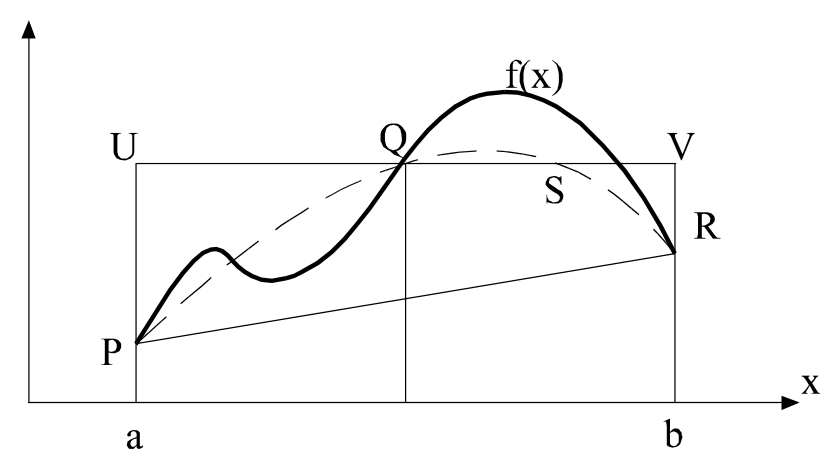
\includegraphics[width = 0.65\textwidth]{../figures/judd_newton_cotes.png}
    \caption{See \cite{judd1998numerical}}
  \end{figure}
\end{minipage}
\end{frame}

\begin{frame}
  \frametitle{Numerical Integration --- Newton Cotes Quadratures}
\alert{\textbf{Midpoint Rule:}}
\begin{itemize}
  \item The simplest quadrature formula with one point given by
  \[
  \int^b_a f(x)dx = \underset{Rule}{\underbrace{(b-a)f\left(\frac{a+b}{2}\right)}} + \underset{Error}{\underbrace{\frac{(b-a)^3}{24}f''(\xi)}}
  \]
  for some $\xi\in [a,b]$. Based on Taylor's theorem and the IVT.
  \item Let $n\geq 1$ be the number of subintervals, $h = (b -a) / n$, and $x_j = a + (j - \frac{1}{2})h$ , $j=1,2,\ldots,n$. The \alert{\textbf{composite midpoint rule}} {\tiny (omitting the error)} is given by
  \[
  \int^b_a f(x)dx = h\sum^n_{j=1}f(x_j) \Rightarrow \text{\alert{\textbf{Same as the Riemann Sum!!}}}
  \]
\end{itemize}
\end{frame}

\begin{frame}[fragile]
  \frametitle{Numerical Integration --- Newton-Cotes Quadratures}
\begin{example}
Compute $\int^5_1 x^2 dx = \frac{124}{3}\approx 41.333$. Errors decline with the number of points $n$.
\end{example}
\begin{columns}
\begin{column}{0.45\textwidth}
\begin{lstlisting}[basicstyle=\footnotesize\ttfamily]
function [value] = midpoint_rule(a,b,n,myfunc)
  % Numerical integration with midpoint rule
  xpts = zeros(n,1);
  h = (b-a)/n;
  for jj=1:n 
      xpts(jj,1) = a + (jj - 1/2)*h;
  end
  value = h*sum(myfunc(xpts));
end
\end{lstlisting}
\end{column}
\begin{column}{0.5\textwidth}
  \begin{figure}
    \centering
    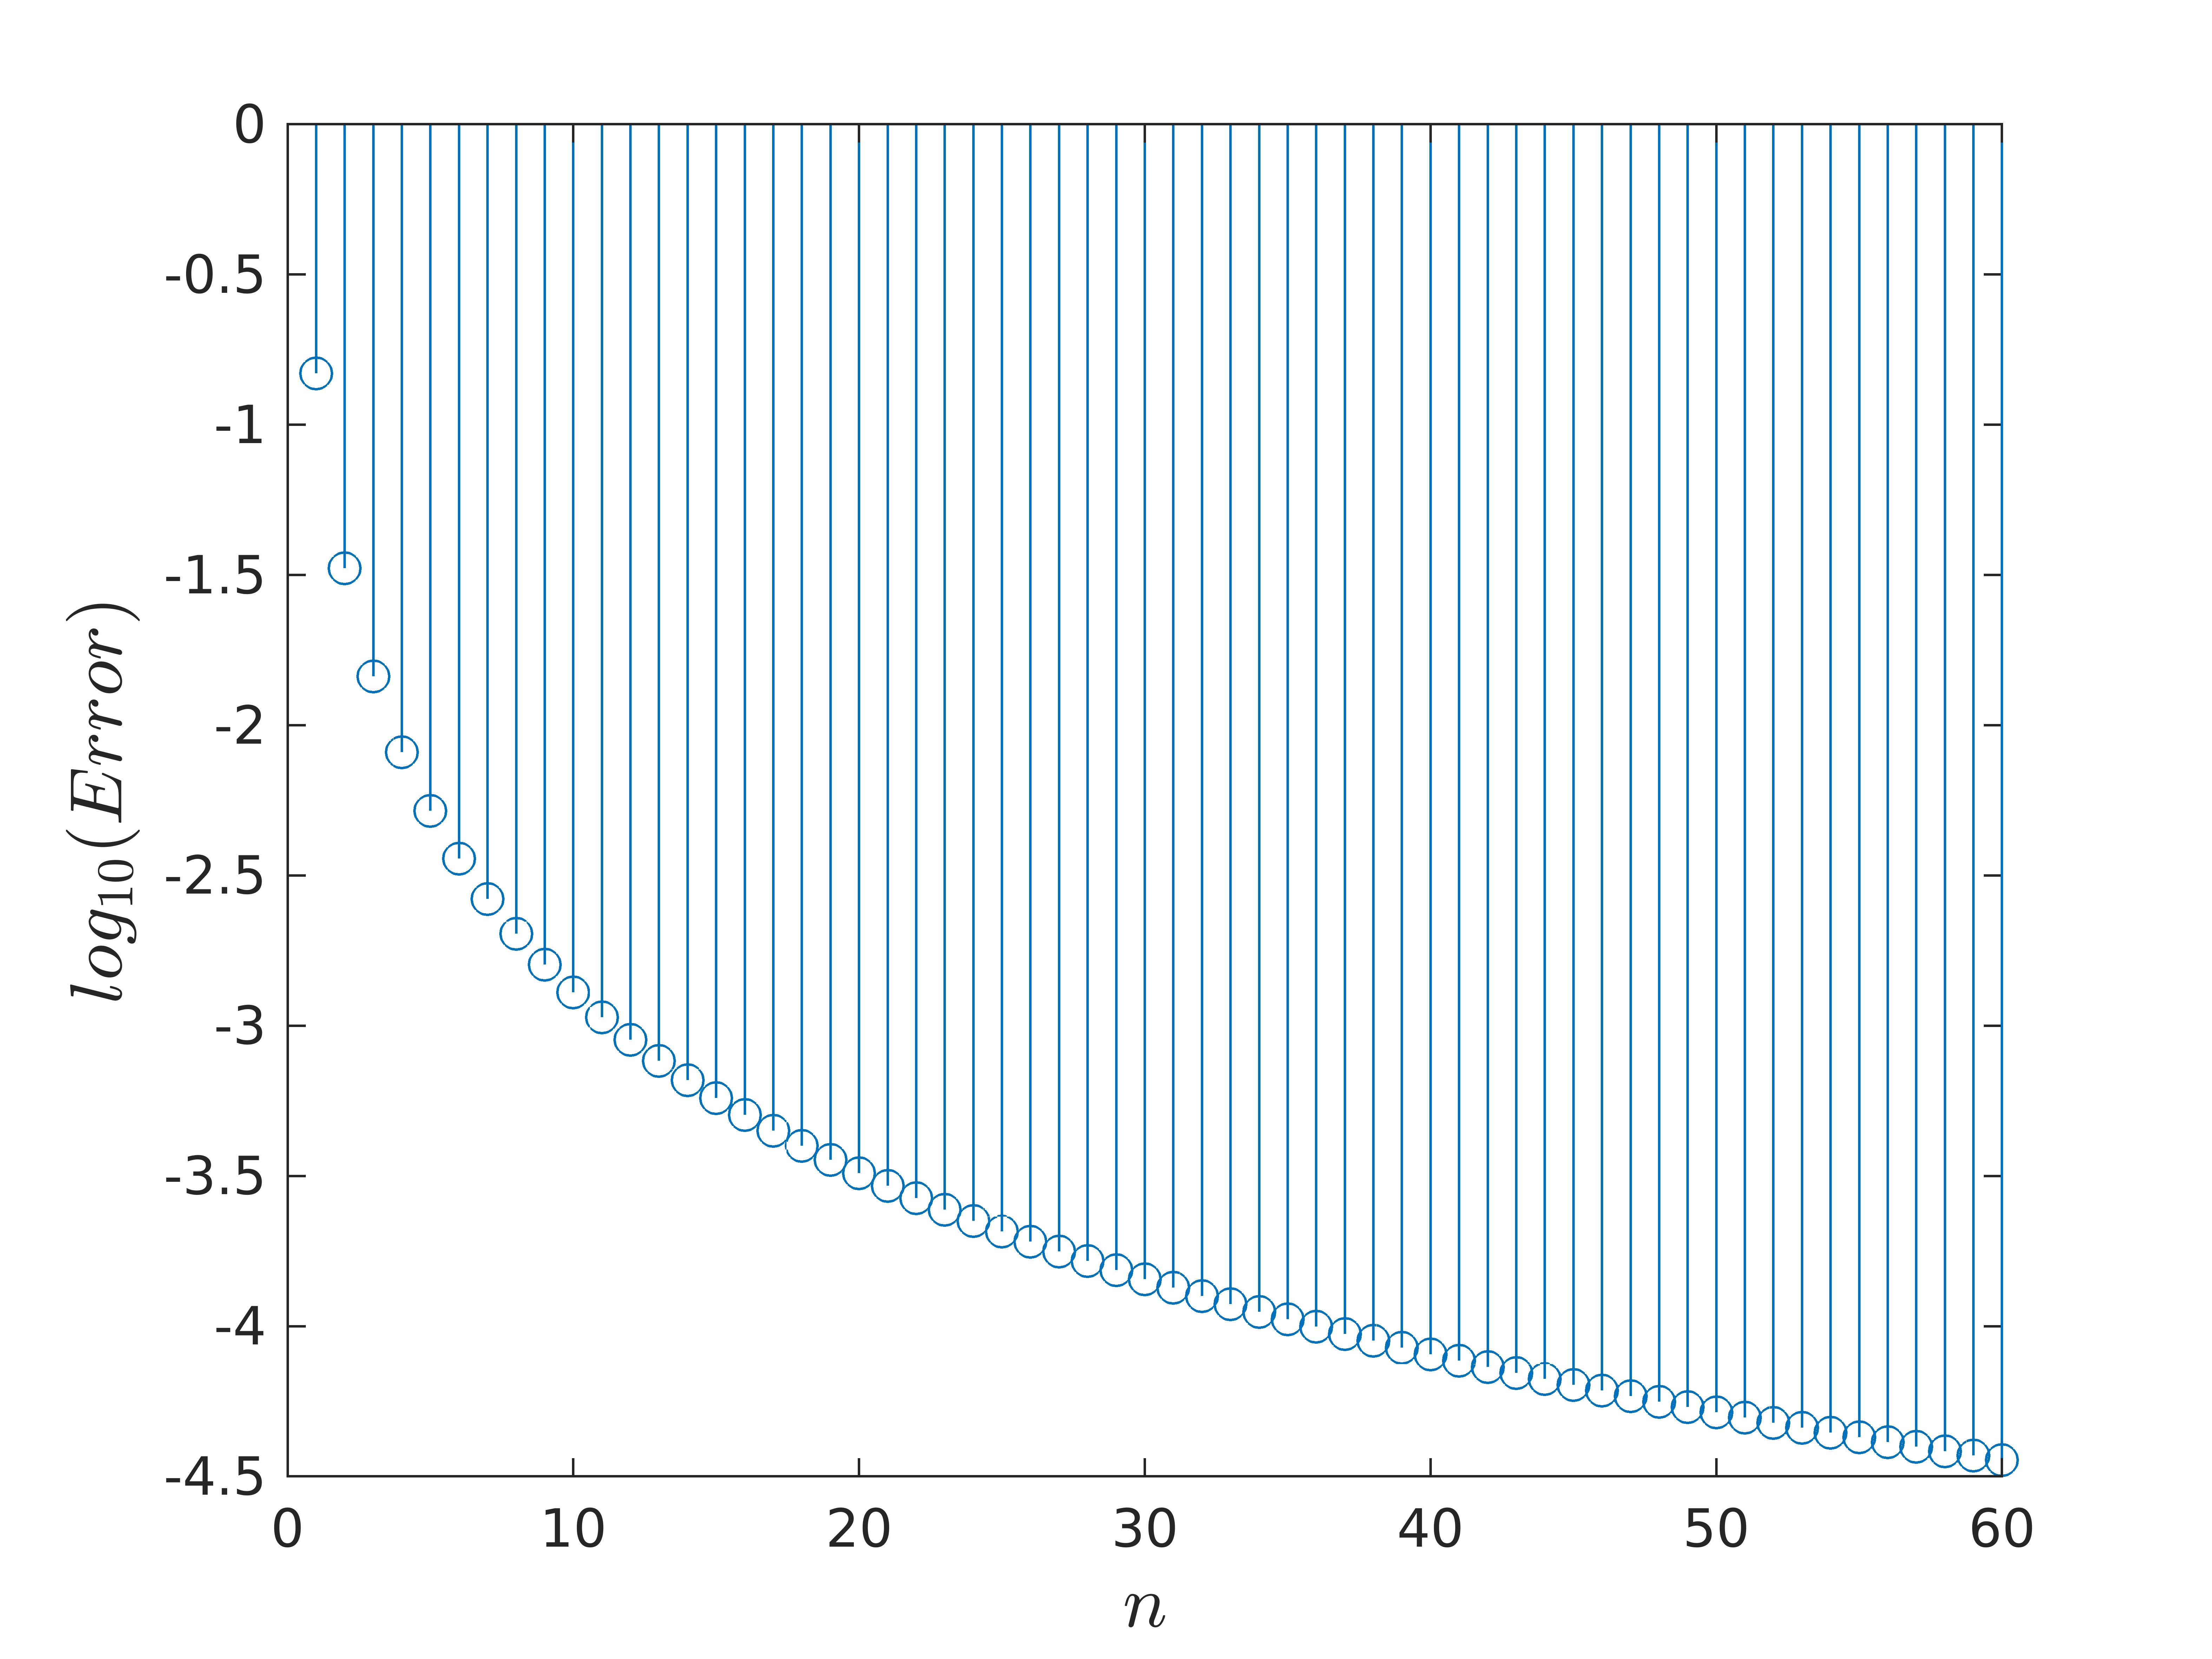
\includegraphics[width=\textwidth]{../figures/errors_midpointrule.png}
    \caption{Relative errors in $\log_{10}$ units}
  \end{figure}
\end{column}
\end{columns}
\end{frame}

\begin{frame}
  \frametitle{Numerical Integration --- Newton-Cotes Quadratures}
  \alert{\textbf{Trapezoid Rule:}}
\begin{itemize}
  \item Use linear approximations of $f$ using the end-points of $[a,b]$.
  \item The rule is
  \[
  \int^b_a f(x)  dx = \frac{b-a}{2}(f(a) + f(b)) - \frac{(b - a)^3}{12}f''(\xi)
  \]
  for some $\xi\in [a,b]$.
  \item Composite trapezoid rule letting $h = (b-a)/n$ and $x_i = a + ih$
  \[
  \int^b_a f(x)dx = \frac{h}{2}\left(f(x_0) + 2f(x_1) + \cdots + 2f(x_{n-1}) + f(x_n)\right)
  \]
\end{itemize}
\end{frame}

\begin{frame}
  \frametitle{Numerical Integration in Matlab}
\begin{itemize}
  \item As with root finding, Matlab has routines for numerical integration.
  \item The trapezoid rule is implemented in \href{https://www.mathworks.com/help/matlab/ref/trapz.html}{\texttt{trapz}} (you'll work with this on the Problem Set).
  \item Another routine is \href{https://www.mathworks.com/help/matlab/ref/integral.html}{\texttt{integral}}.
  \item The latter uses adaptive quadratures. Basically, adapts the subintervals refining the process. But the quadrature rules can still be Newton-Cotes.
  \item For double and triple integrals, Matlab has \href{https://www.mathworks.com/help/matlab/ref/integral2.html}{\texttt{integral2}} and \href{https://www.mathworks.com/help/matlab/ref/integral3.html}{\texttt{integral3}} respectively.
\end{itemize}
\end{frame}

\section{Details on Solution Methods}

\subsection{Details on Bisection Method}

\begin{frame}
  \frametitle{Bisection Method --- Stopping Criteria}
\alert{\textbf{Criterion 1:}}
\begin{itemize}
  \item Parameter $\delta$ controls the \textit{``acceptable error''}.
  \item Sometimes, computing $f(x)$ involves other numerical operations that add errors to the computation of $f$.
  \item We should take that into account when choosing a value for $\delta$
\end{itemize}
\end{frame}


\begin{frame}
  \frametitle{Bisection Method --- Stopping Criteria}
\alert{\textbf{Criterion 2:}}
\begin{itemize}
  \item The size of the interval is too small whenever
  \[
  \frac{x^R - x^L}{(1 + \lvert x^L \rvert + \lvert x^R \rvert)} \leq \varepsilon
  \]
  \item No sense in choosing $\varepsilon = 0$, unachievable. Same for $\varepsilon = 10^{-130}$, computers store finite digits.
  \item Bear in mind the sizes of $x^L$ and $x^R$. {\tiny If $x^L$ and $x^R$ are of the order $10^{10}$, convergence of $x^R-x^L < 10^{-5}$ is infeasible.}
  \item Note that adding $1$ avoids problems when $x^R\approx x^L \approx 0$
\end{itemize}
\end{frame}

\begin{frame}
  \frametitle{Bisection Method --- Stopping Criteria}
\alert{\textbf{Criterion 3:}}
\begin{itemize}
  \item We can compute the minimum number of iterations $N$ to achieve accuracy $\delta$
  \item We want the length of the interval after $N$ iterations lower than $\delta$
  \[
  \frac{x^R - x^L}{2^N} \leq \delta \Rightarrow 2^N \geq \frac{x^R - x^L}{\delta}
  \]
  taking logs on both sides and simplifying
  \[
  N\geq \frac{\log(x^R - x^L) - \log(\delta)}{\log(2)}  
  \]
  which depends on the length of the interval $[x^L, x^R]$ and the value of $\delta$
\end{itemize}
\end{frame}

\begin{frame}
  \frametitle{Bisection Method --- Example}
Compute the positive root of $f(x) = x^3 - 6x^2 + 11x - 6$
\begin{enumerate}
  \item Find the interval $[x^L, x^R]$
  \item The function has three positive roots, let's focus on the one on the interval $[2.5, 4]$
  \item Note $f(2.5)f(4) = -2.25 < 0 \Rightarrow$ by IVT there is a root in $[2.5, 4]$
  \item Choose $\delta = 10^{-4}$ and $\varepsilon = 10^{-8}$
  \item The minimum number of iterations needed to achieve accuracy $\delta$ is $N^{min} = 13.8$, choose $N = N^{min} + 50$
\end{enumerate}
\end{frame}

\begin{frame}[fragile]
  \frametitle{Bisection Method --- The Actual Code}
  \begin{itemize}
    \item Initialize with a \verb;while; loop with three conditionals
\begin{lstlisting}
while (error_f > delta) && (error_i > epsil) && (it < maxit)
% Actual algorithm in here
end     
\end{lstlisting}
    \item Middle steps
\begin{lstlisting}
% Compute xm
xm = xl + (xr - xl) / 2; % Slightly improves performance

% Compute value of f at xm
fxm = myf(xm);

% Compute bounds values of f
fxl = myf(xl);
fxr = myf(xr);
\end{lstlisting}
\end{itemize}
\end{frame}

\begin{frame}[fragile]
  \frametitle{Bisection Method --- The Actual Code}
\begin{itemize}
  \item Compute errors
\begin{lstlisting}
% Compute errors
error_f = abs(fxm);
error_i = (xr - xl)./(1 + abs(xl) + abs(xr));
\end{lstlisting}
\item Update iteration counter and refine interval
\begin{lstlisting}
% Update iteration counter
it = it + 1;

% Update if necessary
if fxm*fxl < 0
    xr = xm;
else
    xl = xm;
end
\end{lstlisting}
\end{itemize}
\end{frame}

\subsection{Details on Newton-Raphson Method}

\begin{frame}
  \frametitle{Newton-Raphson --- Existence, Uniqueness, and Convergence}
\begin{theorem}[Fixed-Point Iteration Theorem]\label{thm:fixed_point}
Let $f(x) = 0$ be written as $x = g(x)$. Let $g(x)$ satisfy:
\begin{enumerate}
  \item $\forall x\in [a,b], g(x)\in [a,b]$
  \item $g'(x)\in (a, b)$ and, for $q\in(0,1)$, $g'(x)$ satisfies $\lvert g'(x) \rvert < q$ for all $x\in (a,b)$
\end{enumerate}
then
\begin{enumerate}
  \item $\exists! c\in(a,b) : g(c) = c$ {\footnotesize \alert{\textbf{(Existence of a unique solution)}}}
  \item For any $x_0\in [a, b]$, the sequence $\{x_k\}$ defined by
  \[
  x_{k+1} = g(x_k) \ , \ k = 0,1,\ldots
  \]
  converges to the fixed point $c = g(c)$, that is to the root $c$ of $f(x) = 0$.
\end{enumerate}
\end{theorem}
\end{frame}

\begin{frame}
  \frametitle{Newton-Raphson Method --- Example}
As with the bisection method, let's compute the root of $f(x) = x^3 - 6x^2 + 11x - 6$ in the interval $[2.5, 4]$. Keep the same stopping criteria parameters.
\begin{enumerate}
  \item Choose $N = 64, \delta = 10^{-4},$ and $\varepsilon = 10^{-8}$
  \item Choose $x_0 = 2.65$.
\end{enumerate}
\end{frame}

\begin{frame}[fragile]
  \frametitle{Newton-Raphson Method --- The Actual Code}
  \begin{itemize}
    \item Initialize with a \verb;while; loop with three conditionals as in bisection
\begin{lstlisting}
while (error_f > delta) && (error_i > epsil) && (it < maxit)
% Actual algorithm in here
end     
\end{lstlisting}
    \item Middle steps
\begin{lstlisting}
% Compute next guess
xkp = xk - myf(xk) ./ fprime(xk);
    
% Compute the errors at current guess
error_f = abs(myf(xk));
error_i = abs(xk - xkp) ./ (1 + abs(xkp));

% Update iteration counter and guess
it = it+1;
xk = xkp;
\end{lstlisting}
\end{itemize}
\end{frame}

\begin{frame}
  \frametitle{Newton-Raphson vs Bisection}
\begin{itemize}
  \item In previous example, it took $14$ iterations for the bisection method to find a solution.
  \item It took Newton-Raphson \alert{\textbf{half}} of those. In $7$ iterations it was done.
  \item Both achieved the same solution.
  \item Note that the first guess for bisection yields $x^M = 3.25$. If we start Newton-Raphson with that guess, only $4$ iterations are needed.
  \item If we give Newton-Raphson $x_0 = 2.5$, we end up in the root $x^* = 1$.
  \item Both methods have pros and cons. It depends on the problem which one to choose.
\end{itemize}
\end{frame}

\end{document}
